\documentclass{cumcmthesis_v3}

\usepackage[framemethod=TikZ]{mdframed}
\usepackage{url}
\usepackage{subcaption}
\usepackage{color}
\usepackage[noend]{algpseudocode}
\usepackage{algorithmicx,algorithm}
\usepackage{tikz}
\usetikzlibrary{arrows.meta,positioning,fit,backgrounds}
\usepackage{graphicx}
\usepackage{lastpage}
\usepackage{fancyhdr}
\usepackage{amsmath}
\usepackage{pdflscape}

\pagestyle{fancy}
\numberwithin{figure}{section}
\numberwithin{table}{section}

\titlename{祈祷一个好头}
\email{黄羽霖、脱晓颖}
\yearinput{2026}
\monthinput{07}
\dayinput{20}

\fancyhead[L]{}
\fancyhead[R]{}
\fancyhead[C]{\zihao{-5} 基于 SEEG 的癫痫发作状态智能检测算法方案}
\fancyfoot[C]{\zihao{-5} 第\thepage 页 \enspace 共 \pageref{LastPage} 页}
\renewcommand{\headrulewidth}{0.5pt}

\newcommand{\makeothertitle}{}

\begin{document}
\normalem
\maketitle

\newpage
\thispagestyle{empty}
\tableofcontents
\newpage

\thispagestyle{empty}
\listoffigures
\newpage

\thispagestyle{empty}
\listoftables
\newpage

\setcounter{page}{1}

\begin{cnabstract}
本方案面向多通道立体定向脑电图（SEEG）癫痫发作状态检测任务，目标是完成片段分类、发作概率估计、发作起始时刻（onset）定位和 Top-10 重要通道排序。方案采用一条可直接实现的基础链路：首先对信号进行患者级数据审计、滤波、坏道处理和稳健标准化；随后使用共享时域卷积与短时傅里叶变换（STFT）提取每个通道的波形和频谱特征；再通过轻量门控融合和时序卷积网络（TCN）建模发作从背景到持续异常的演化；最后由片段状态、帧级状态、onset 边界和通道贡献四个输出头生成比赛结果。

onset 不由单个阈值瞬间决定，而是结合状态概率持续上升、边界峰值和最短持续时间进行判定，以减少孤立尖波和伪迹造成的误触发。正式 Top-10 按模型贡献度、遮挡验证和跨折稳定性排序，不直接等同于临床发作起始区（SOZ）或致痫区（EZ）。动态图、Morlet 小波、电极坐标和脑区映射均列为数据与验证条件满足后才启用的增强模块，不进入第一版基础系统。训练、校准和模型选择均以患者为隔离单位，并以官方指标和目标硬件端到端时延作为最终依据。

\cnkeywords{SEEG \quad 癫痫发作检测 \quad onset 定位 \quad 重要通道排序 \quad 时频分析 \quad TCN \quad 医学人工智能}
\end{cnabstract}

\section*{研究背景与任务理解}
\addcontentsline{toc}{section}{研究背景与任务理解}

癫痫发作的 SEEG 表现并不只有一种固定波形。部分发作以低电压快速活动开始，部分表现为节律性尖波、低频周期性放电或逐渐演化的频谱变化\cite{abdallah_sop}。同时，发作间期也可能出现孤立棘波、尖波和高频振荡。因此，模型不能把“某一帧振幅很大”简单等同于“已经发作”，而应观察异常是否持续、是否发生状态转变以及是否在多个时间帧中形成一致证据。

本方案服务于比赛任务，而不是直接作出临床手术结论。模型给出的 Top-10 是对当前片段判定最重要的已植入通道；SOZ 是临床判读认为最早出现发作性电活动的区域；EZ 是为获得无发作结局需要处理的理论组织范围。三者并不等价\cite{rosenow_ez}。模型结果必须结合原始波形、影像和多学科评估解释。

\section{任务目标与总体方案}

\subsection{需要完成的四项输出}

根据任务要求，系统对每个样本生成表~\ref{tab:outputs} 所列结果。本文所有模型设计都围绕这四项输出展开，不为增加复杂度而引入与任务无关的模块。

\begin{table}[htbp]
\centering
\zihao{5}
\caption{比赛输出及本方案的实现方式}
\label{tab:outputs}
\renewcommand{\arraystretch}{1.35}
\begin{tabularx}{\linewidth}{@{}p{0.18\linewidth}p{0.31\linewidth}X@{}}
\toprule
\textbf{输出} & \textbf{含义} & \textbf{实现方式} \\
\midrule
片段标签 & 片段是否包含发作 & 由片段状态概率按验证集阈值转换 \\
发作概率 & 模型对阳性片段的置信度 & 对帧级状态序列聚合后进行折外校准 \\
onset & 阳性片段内的发作起始时间 & 联合状态上升、边界峰值和持续时间确定 \\
Top-10 通道 & 对当前判断贡献最大的通道 & 根据通道贡献、遮挡下降和跨折稳定性排序 \\
\bottomrule
\end{tabularx}
\end{table}

\subsection{一条可以直接实现的默认链路}

默认系统只包含五个步骤：数据预处理、共享特征编码、时域与时频融合、长程时序建模和多任务输出。其数据流如图~\ref{fig:v3-architecture} 所示。

\clearpage
\begin{landscape}
\begin{figure}[p]
\centering
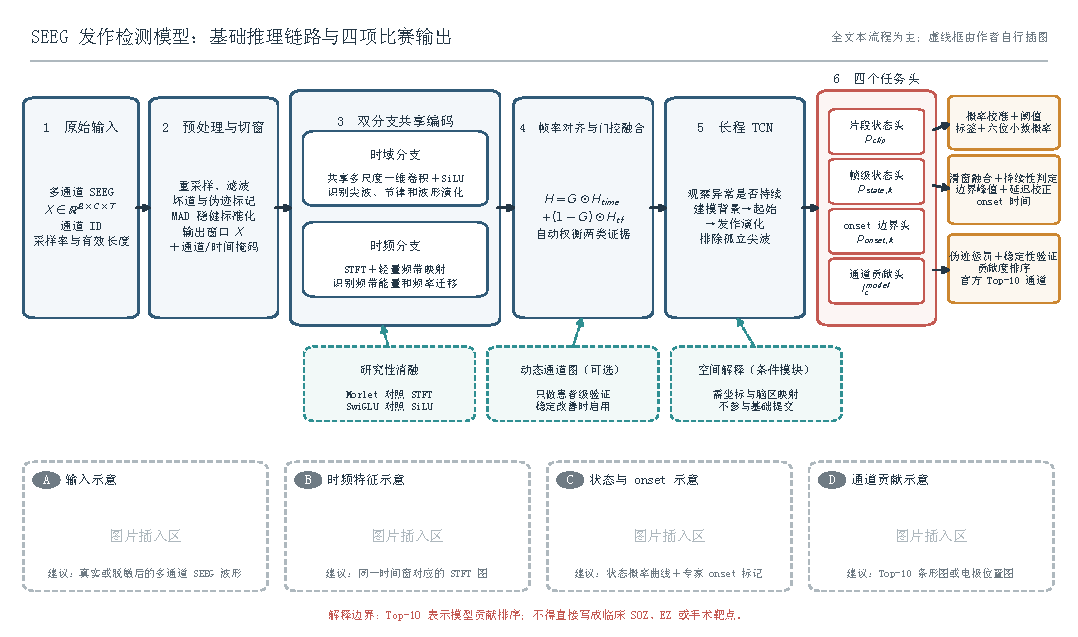
\includegraphics[width=0.98\linewidth,height=0.82\textheight,keepaspectratio]{tmp/pdfs/seeg_figures_zh_final_v3/text-flow-with-placeholders-v1.pdf}
\caption{SEEG 发作检测模型的全文本推理流程、四项比赛输出和候选增强模块。下方四个虚线框为作者预留的图片插入区域。}
\label{fig:v3-architecture}
\end{figure}
\end{landscape}
\clearpage

这张图应按从左到右的顺序理解。输入是经过预处理的多通道 SEEG；共享编码器分别读取每个通道，提取局部波形和频谱变化；TCN 观察这些变化是否持续并形成发作演化；最后四个输出头分别完成片段判断、逐帧判断、onset 定位和通道排序。模型名称只用于称呼该整体结构，不代表必须同时启用所有候选模块。

\subsection{基础模块与可选模块的边界}

\begin{table}[htbp]
\centering
\zihao{5}
\caption{模块优先级与启用条件}
\label{tab:module-priority}
\renewcommand{\arraystretch}{1.35}
\begin{tabularx}{\linewidth}{@{}p{0.20\linewidth}p{0.40\linewidth}X@{}}
\toprule
\textbf{层级} & \textbf{模块} & \textbf{处理原则} \\
\midrule
必须实现 & 时域卷积、STFT、门控融合、TCN、四个输出头 & 构成第一版可训练、可推理、可提交系统 \\
验证后启用 & onset 边界专项监督、通道遮挡训练、动态图 & 只有患者级重复验证稳定改善时保留 \\
条件模块 & 电极坐标、接点--脑区映射、跨发作空间汇总 & 只有数据完整且质控通过时启用 \\
研究性消融 & Morlet 小波、SwiGLU、轻量注意力 & 用于比较，不写成必然优于基线 \\
\bottomrule
\end{tabularx}
\end{table}

\section{数据处理与质量控制}

\subsection{先审计数据，再确定参数}

在确定采样率、窗口长度和模型容量前，先统计患者数、样本数、每位患者的发作次数、通道数、采样率、片段长度、幅值单位、缺失比例和 onset 标注精度。若比赛数据说明与本文假设不一致，以官方数据说明和评测脚本为准。

训练集、验证集和测试集必须按患者隔离。同一患者的不同片段不能跨集合，否则模型可能记住患者、设备或植入方式，得到虚高结果。还需使用文件哈希、降采样波形和频谱相似度排查同一连续记录产生的近重复片段。

\subsection{滤波、重采样与坏道处理}

重采样目标由原始采样率决定。若原始数据支持且高频信息在患者级验证中有效，可统一到 512 Hz；否则采用 256 Hz 以降低计算量。任何分析频率都必须低于重采样后的奈奎斯特频率。工频根据功率谱自动识别为 50 Hz 或 60 Hz，并在必要的谐波处抑制。

坏道检测综合使用平线比例、饱和比例、异常方差、工频占比和宽带尖峰密度。坏道不直接删除，而是保留独立掩码，确保模型知道该通道当前不可用。滤波产生的群延迟、滑窗中心偏移和补齐区域必须在 onset 输出时统一校正。

\subsection{稳健标准化}

SEEG 中可能存在幅值很大的尖峰和伪迹，普通均值与标准差容易被少数极端值带偏。因此，每个通道采用中位数和中位绝对偏差（MAD）标准化：

\[
\operatorname{MAD}(x_c)=
\operatorname{median}_t\left|x_{c,t}-\operatorname{median}_t(x_{c,t})\right|,
\]

\[
\tilde{x}_{c,t}=\operatorname{clip}\left(
\frac{x_{c,t}-\operatorname{median}(x_c)}
{1.4826\operatorname{MAD}(x_c)+\varepsilon},-q,q\right).
\]

第一式计算通道波形相对中位数的典型偏差。对于正态分布，MAD 约为标准差的 $0.6745$ 倍，因此乘以 $1/0.6745\approx1.4826$ 后可得到与标准差相近的稳健尺度。最后的截断把极端伪迹限制在 $[-q,q]$ 内。若软件库已经返回正态校准后的 MAD，则不再重复乘 $1.4826$。

\subsection{滑动窗口和标签对齐}

长片段采用重叠滑窗推理。窗口必须覆盖发作前背景和早期演化，但不能长到严重增加时延。初始可从 8～16 秒窗口、50\% 重叠开始，再按训练数据调整。窗口末端补齐区域使用时间掩码，不参与损失和 onset 搜索。

onset 标签首先服从官方定义。若官方只给出一个时间值而未说明其对应“最早可疑变化”“最早明确电图变化”还是“首批通道持续募集”，则将其视为数据集的操作性边界，不擅自解释成真实 EZ 启动时刻。

\section{发作状态识别模型}

\subsection{共享时域编码器}

每个通道使用同一套一维卷积参数。短、中、长三种感受野分别观察尖波、局部节律和较慢的波形演化。共享参数使模型学习“什么波形像发作”，而不是记忆某个患者的固定通道编号。卷积主干使用 SiLU 激活；SwiGLU 只在前馈子层进行等参数消融，不作为默认替换。

\subsection{STFT 时频分支}

STFT 将波形转换为“时间--频率--能量”表示，用于观察某个频带是否持续增强、频率是否迁移以及是否存在工频污染。正式基线使用 STFT 或多分辨率 STFT，因为它便于缓存、部署和解释。Morlet 小波只用于比较短暂高频活动的识别效果，验证没有稳定收益时不进入正式模型。

\subsection{门控融合}

时域分支擅长识别波形形态，时频分支擅长识别频谱演化。模型使用门控权重决定当前更依赖哪类证据：

\[
H_{c,k}=G_{c,k}\odot H^{\mathrm{time}}_{c,k}
+(1-G_{c,k})\odot H^{\mathrm{tf}}_{c,k}.
\]

其中，$G_{c,k}$ 的取值位于 0 和 1 之间。$G$ 越大，模型越重视时域波形；$G$ 越小，模型越重视频谱特征。该公式的作用只是加权融合两类信息，不表示两个分支具有临床因果关系。

\subsection{TCN 与四个输出头}

融合特征送入扩张 TCN。TCN 的作用是观察异常是否持续以及是否从背景逐步演化为发作，从而区别孤立尖波和真正的发作过程。模型设置四个输出头：

\begin{itemize}[leftmargin=2em,itemsep=0.3em]
\item 片段状态头：输出整个片段的发作概率；
\item 帧级状态头：输出每个时间帧处于发作状态的概率；
\item onset 边界头：输出每个时间帧成为状态转折点的概率；
\item 通道贡献头：输出每个通道对当前判断的快速贡献分数。
\end{itemize}

动态图不属于默认链路。只有在不含动态图的基线已经稳定后，才比较动态图能否利用通道间的统计领先关系进一步改善结果。动态图输出只能解释为关联或传播上游候选，不能直接称为因果传播。

\subsection{训练目标}

总损失采用易于解释的加权和：

\[
\mathcal{L}=\lambda_1\mathcal{L}_{\mathrm{clip}}
+\lambda_2\mathcal{L}_{\mathrm{frame}}
+\lambda_3\mathcal{L}_{\mathrm{onset}}
+\lambda_4\mathcal{L}_{\mathrm{channel}}.
\]

四项损失分别监督片段标签、帧级状态、onset 边界和通道贡献。若训练数据没有帧级或通道级标注，对应损失通过掩码关闭，不能用测试标注或人工猜测补齐。权重在训练折内确定，不根据最终测试结果反复调整。

\section{发作起始点定位}

\subsection{模型需要寻找的 onset}

医学判读中，“最早可疑变化”“最早明确电图变化”“首批通道持续募集”和“首次临床症状”可能对应不同时间点。本系统的监督目标首先采用官方 onset 标注。模型定位的是数据集定义的操作性边界，而不是声称找到了真实 EZ 的启动时刻。

\subsection{从逐帧概率得到唯一时间点}

长片段使用重叠滑窗后，同一时间点会得到多个预测。系统先使用 Hann 权重融合这些预测，重建连续的状态概率 $p_k$ 和边界概率 $b_k$。然后按图~\ref{fig:v3-onset} 完成判定。

\begin{figure}[htbp]
\centering
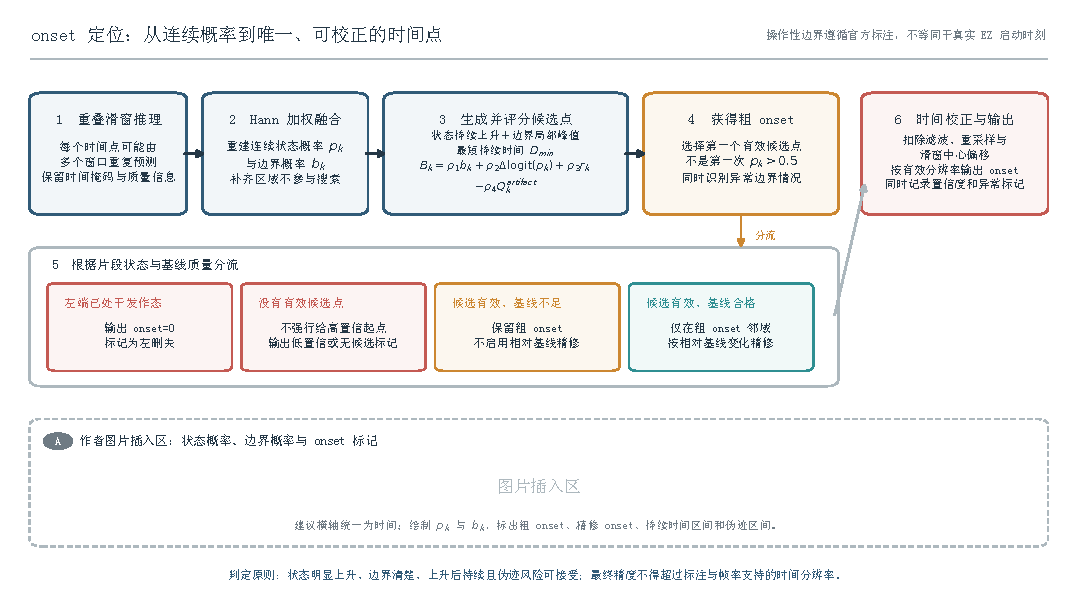
\includegraphics[width=\linewidth]{tmp/pdfs/seeg_figures_zh_final_v3/onset-flow-current-v1.pdf}
\caption{V3 onset 定位流程：融合连续概率、生成并评分候选点，根据边界情况与基线质量分流，最后完成时间校正。下方虚线框为作者预留的概率曲线插入区。}
\label{fig:v3-onset}
\end{figure}

第一步寻找状态概率持续上升的候选区间，而不是把第一次 $p_k>0.5$ 直接作为 onset。第二步在候选区间内寻找边界概率峰值。第三步要求发作状态至少持续 $D_{\min}$，用于排除孤立尖峰。候选点可采用下式评分：

\[
B_k=\rho_1 b_k+
\rho_2\Delta\operatorname{logit}(p_k)+
\rho_3 r_k-
\rho_4 Q_k^{\mathrm{artifact}}.
\]

其中，$b_k$ 表示边界证据，$\Delta\operatorname{logit}(p_k)$ 表示状态概率上升速度，$r_k$ 表示早期通道异常强度，$Q_k^{\mathrm{artifact}}$ 表示伪迹风险。该公式的目的，是在多个候选点中选择“状态明显上升、边界清楚、通道证据存在且伪迹较少”的第一个有效点。

\subsection{两阶段推理与异常情况}

第一阶段只使用默认时域--时频模型获得粗 onset。若粗 onset 前存在足够长且质量合格的背景区间，第二阶段才计算相对基线变化，并在限定邻域内精修 onset。若片段左侧已经处于高概率发作状态，则输出 onset 为 0，并标记为左删失；若没有任何候选点满足持续性条件，则不强行输出高置信度起点。

最终时间还需扣除滤波群延迟、重采样延迟和滑窗中心偏移。模型报告的精度不能高于数据标注和输出帧率实际支持的时间分辨率。

\section{Top-10 重要通道排序}

\subsection{正式提交采用模型贡献度}

比赛 Top-10 的问题是：“哪些通道对当前模型判断最重要？”默认通道分数写为：

\[
S_c^{\mathrm{comp}}=
\alpha I_c^{\mathrm{model}}+
\beta I_c^{\mathrm{occlusion}}+
\gamma I_c^{\mathrm{stability}}-
\eta Q_c^{\mathrm{artifact}}.
\]

$I_c^{\mathrm{model}}$ 是一次前向得到的快速贡献分数；$I_c^{\mathrm{occlusion}}$ 表示遮挡该通道后发作概率下降多少；$I_c^{\mathrm{stability}}$ 表示该通道在不同训练折和轻微扰动下是否仍保持较高排名；$Q_c^{\mathrm{artifact}}$ 用于降低坏道和严重伪迹通道的分数。正式推理优先使用快速贡献分数，遮挡和稳定性主要用于离线验证及少量低置信度病例复核。

遮挡时不直接把整条波形突然置零，以免制造非生理阶跃。优先在特征层遮挡，或用发作前基线、频谱匹配噪声替换，并保留独立缺失掩码。

\subsection{临床早期通道只作附加解释}

“最早出现持续异常的通道”与“对模型分类最重要的通道”可能不同。晚期传播通道振幅更大，可能具有很高的分类贡献，但并不是最早募集通道。因此，临床探索性排序只在附加报告中给出，综合首次持续异常时间、相对基线变化和演化持续性，不直接替代官方 Top-10。

无论哪种排序，结果都只覆盖已植入电极记录到的范围，不直接命名为 SOZ、EZ 或手术靶点。

\section{训练、验证与模型选择}

\subsection{患者级实验设计}

数据按患者划分训练、验证和外层测试。若患者数量允许，采用患者级嵌套交叉验证；若患者较少，则采用患者级留一法或分组交叉验证。所有标准化统计量、类别权重、阈值和校准器均只能使用训练折或折外预测得到。

模型选择首先服从官方评价指标。若官方综合指标尚未公开，暂以患者级宏平均 PR-AUC 为主要分类指标，并同时报告 F1、ROC-AUC、灵敏度、特异度和校准误差。onset 单独报告 MAE、平均有符号误差以及 $\pm1$ s、$\pm3$ s 命中率。Top-10 报告遮挡后性能下降、仅保留 Top-10 后的性能保持率和跨折 Jaccard 稳定性。

\subsection{按顺序增加模块}

实验不一次性训练全部模块，而按表~\ref{tab:ablation-v3} 的顺序逐步增加。只有一个模块在患者级重复实验中产生稳定收益，且没有明显增加时延或降低校准质量时，才保留到下一阶段。

\begin{table}[htbp]
\centering
\zihao{5}
\caption{V3 分阶段消融顺序}
\label{tab:ablation-v3}
\renewcommand{\arraystretch}{1.35}
\begin{tabularx}{\linewidth}{@{}p{0.13\linewidth}p{0.36\linewidth}X@{}}
\toprule
\textbf{阶段} & \textbf{模型} & \textbf{目的} \\
\midrule
M0 & 时域卷积＋全局池化 & 建立最简单分类基线 \\
M1 & M0＋STFT＋门控融合 & 验证频谱信息是否提供稳定增益 \\
M2 & M1＋TCN＋帧级状态 & 验证持续性建模和 onset 基础能力 \\
M3 & M2＋onset 边界头 & 验证专项边界监督是否优于概率后处理 \\
M4 & M3＋通道忠实性验证 & 提高 Top-10 的必要性和稳定性 \\
M5 & M4＋动态图或空间模块 & 仅在基础系统稳定后验证高级模块 \\
\bottomrule
\end{tabularx}
\end{table}

需要重点比较的替代方案只有两组：STFT 与 STFT＋Morlet，SiLU 与前馈层 SwiGLU。比较时保持患者划分、参数量和训练预算尽可能一致。未获得稳定收益的替代项不进入最终提交模型。

\subsection{概率校准}

发作概率需要具有可比较性。校准器只能使用患者级折外 logits 拟合，外层测试患者不能参与校准。比较温度缩放和保序回归后，选择折外 Brier 分数或期望校准误差更低的方法。最终分类阈值同样在训练折内确定。

\section{推理、部署与实施计划}

\subsection{推理流程}

正式推理依次执行：读取与审计、重采样和滤波、稳健标准化、滑窗批量推理、窗口概率融合、onset 判定、Top-10 排序、概率校准和格式检查。端到端时延从样本读取开始，到最终结果写出结束，不能只报告神经网络前向时间。

GPU 上采用混合精度、批量滑窗和 STFT 缓存；CPU 上采用线程数受控的卷积与 FFT，并通过 ONNX Runtime 或同类后端验证数值一致性。积分梯度、逐通道完整遮挡和动态图深度分析不进入基础低时延链路。

\subsection{阶段性实施计划}

\begin{table}[htbp]
\centering
\zihao{5}
\caption{实施阶段、交付物与继续条件}
\label{tab:milestones-v3}
\renewcommand{\arraystretch}{1.35}
\begin{tabularx}{\linewidth}{@{}p{0.17\linewidth}p{0.33\linewidth}X@{}}
\toprule
\textbf{阶段} & \textbf{主要交付物} & \textbf{继续条件} \\
\midrule
数据审计 & 数据字典、患者级划分、近重复与标签报告 & 未发现无法解释的泄漏或标注冲突 \\
基础基线 & M0/M1 训练代码、患者级指标和错误样例 & 明显优于元数据及简单能量基线 \\
时序与 onset & M2/M3、逐帧曲线和 onset 误差分析 & 多折改善且系统性早晚偏差可解释 \\
通道排序 & 遮挡验证、稳定性和伪迹敏感性报告 & Top-10 在必要性和稳定性上达标 \\
部署冻结 & 固定预处理、权重、校准器和提交检查脚本 & 目标硬件时延与输出格式符合要求 \\
\bottomrule
\end{tabularx}
\end{table}

所有实验保存配置、随机种子、患者划分、代码版本、环境版本和模型校验值。任何性能数字只有在明确患者级划分、数据来源和评价指标后才写入最终报告。

\section{方案优势、风险与责任边界}

本方案的主要优势不是模块数量，而是任务对应清楚：分类由片段状态完成，onset 由逐帧状态和边界证据完成，Top-10 由经过遮挡验证的通道贡献完成；高级模块只有验证有效才启用。共享通道编码和患者级隔离降低模型记忆固定植入布局的风险，持续性约束减少孤立尖波误报，分层推理兼顾速度和解释深度。

主要风险包括患者数量不足、onset 标注标准不一致、类别严重不平衡、伪迹被误识别为发作以及复杂模块过拟合。对应措施分别是分组交叉验证、标注审计、患者--类别均衡采样、坏道与伪迹质量分数以及预先规定的模块退出条件。

系统属于比赛算法和临床决策支持研究。输出应附带置信度、质量标记和波形证据，不在没有医生复核的情况下用于诊断、切除范围制定或设备自动刺激。

\addcontentsline{toc}{section}{参考文献}
\begin{thebibliography}{99}
\bibitem{who_epilepsy} World Health Organization. Epilepsy fact sheet[EB/OL]. \url{https://www.who.int/news-room/fact-sheets/detail/epilepsy}.
\bibitem{kwan_dre} Kwan P, Arzimanoglou A, Berg A T, et al. Definition of drug resistant epilepsy: consensus proposal by the ILAE Commission on Therapeutic Strategies[J]. Epilepsia, 2010, 51(6): 1069--1077.
\bibitem{alomar_seeg} Alomar S, Jones J, Maldonado A, et al. The stereo-electroencephalography methodology[J]. Neurosurgery Clinics of North America, 2016, 27(1): 83--95.
\bibitem{abdallah_sop} Abdallah C, Mansilla D, Minato E, et al. Systematic review of seizure-onset patterns in stereo-electroencephalography[J]. Clinical Neurophysiology, 2024, 163: 112--123.
\bibitem{bartolomei_ei} Bartolomei F, Chauvel P, Wendling F. Epileptogenicity of brain structures in human temporal lobe epilepsy[J]. Brain, 2008, 131(7): 1818--1830.
\bibitem{balatskaya_cei} Balatskaya A, Roehri N, Lagarde S, et al. The Connectivity Epileptogenicity Index[J]. Clinical Neurophysiology, 2020, 131(8): 1947--1955.
\bibitem{hfo_review} Lee S, Issa N P, Rose S, et al. DC shifts, high frequency oscillations, ripples and fast ripples in relation to the seizure onset zone[J]. Seizure, 2020, 77: 52--58.
\bibitem{rosenow_ez} Rosenow F, L\"uders H. Presurgical evaluation of epilepsy[J]. Brain, 2001, 124(9): 1683--1700.
\bibitem{competition_page} 赛题组委会. 脑机接口：基于 SEEG 的癫痫发作状态智能检测[EB/OL]. \url{https://www.aicompetition-pz.com/topic_detail/34}.
\end{thebibliography}

\clearpage
\section*{附录 A：术语速查}
\addcontentsline{toc}{section}{附录 A：术语速查}

\begin{table}[htbp]
\centering
\zihao{5}
\renewcommand{\arraystretch}{1.35}
\begin{tabularx}{\linewidth}{@{}p{0.20\linewidth}X@{}}
\toprule
\textbf{术语} & \textbf{本文中的含义} \\
\midrule
SEEG & 植入脑内电极记录的多通道局部电活动 \\
onset & 官方标注定义的片段内发作起始时间 \\
募集 & 某个通道开始出现持续发作样异常的过程 \\
传播 & 异常活动在更多已记录通道中出现的过程 \\
SOZ & 临床认为最早出现发作性电活动的区域 \\
EZ & 为获得无发作结局需要处理的理论组织范围 \\
Top-10 & 对比赛模型当前判断贡献最大的十个通道 \\
TCN & 使用扩张一维卷积建模长时间依赖的时序网络 \\
MAD & 中位绝对偏差，用于不易受极端值影响的尺度估计 \\
\bottomrule
\end{tabularx}
\end{table}

\section*{附录 B：提交前检查}
\addcontentsline{toc}{section}{附录 B：提交前检查}

\begin{enumerate}[leftmargin=2em,itemsep=0.3em]
\item 患者是否在训练、验证和测试集合之间严格隔离；
\item 所有预处理参数和校准器是否只使用训练折信息；
\item onset 是否已扣除滤波、重采样和滑窗产生的系统延迟；
\item 补齐时间和补齐通道是否被掩码排除；
\item Top-10 是否使用官方通道 ID，且未被表述为 EZ；
\item 概率位数、字段名称、排序和异常值是否满足官方模板；
\item 端到端时延是否包含读取、预处理、推理和结果写出；
\item 最终模型是否能够由冻结配置和环境完整复现。
\end{enumerate}


\end{document}
